\documentclass[11pt]{article}

    \usepackage[breakable]{tcolorbox}
    \usepackage{parskip} % Stop auto-indenting (to mimic markdown behaviour)
    

    % Basic figure setup, for now with no caption control since it's done
    % automatically by Pandoc (which extracts ![](path) syntax from Markdown).
    \usepackage{graphicx}
    % Keep aspect ratio if custom image width or height is specified
    \setkeys{Gin}{keepaspectratio}
    % Maintain compatibility with old templates. Remove in nbconvert 6.0
    \let\Oldincludegraphics\includegraphics
    % Ensure that by default, figures have no caption (until we provide a
    % proper Figure object with a Caption API and a way to capture that
    % in the conversion process - todo).
    \usepackage{caption}
    \DeclareCaptionFormat{nocaption}{}
    \captionsetup{format=nocaption,aboveskip=0pt,belowskip=0pt}

    \usepackage{float}
    \floatplacement{figure}{H} % forces figures to be placed at the correct location
    \usepackage{xcolor} % Allow colors to be defined
    \usepackage{enumerate} % Needed for markdown enumerations to work
    \usepackage{geometry} % Used to adjust the document margins
    \usepackage{amsmath} % Equations
    \usepackage{amssymb} % Equations
    \usepackage{textcomp} % defines textquotesingle
    % Hack from http://tex.stackexchange.com/a/47451/13684:
    \AtBeginDocument{%
        \def\PYZsq{\textquotesingle}% Upright quotes in Pygmentized code
    }
    \usepackage{upquote} % Upright quotes for verbatim code
    \usepackage{eurosym} % defines \euro

    \usepackage{iftex}
    \ifPDFTeX
        \usepackage[T1]{fontenc}
        \IfFileExists{alphabeta.sty}{
              \usepackage{alphabeta}
          }{
              \usepackage[mathletters]{ucs}
              \usepackage[utf8x]{inputenc}
          }
    \else
        \usepackage{fontspec}
        \usepackage{unicode-math}
    \fi

    \usepackage{fancyvrb} % verbatim replacement that allows latex
    \usepackage{grffile} % extends the file name processing of package graphics
                         % to support a larger range
    \makeatletter % fix for old versions of grffile with XeLaTeX
    \@ifpackagelater{grffile}{2019/11/01}
    {
      % Do nothing on new versions
    }
    {
      \def\Gread@@xetex#1{%
        \IfFileExists{"\Gin@base".bb}%
        {\Gread@eps{\Gin@base.bb}}%
        {\Gread@@xetex@aux#1}%
      }
    }
    \makeatother
    \usepackage[Export]{adjustbox} % Used to constrain images to a maximum size
    \adjustboxset{max size={0.9\linewidth}{0.9\paperheight}}

    % The hyperref package gives us a pdf with properly built
    % internal navigation ('pdf bookmarks' for the table of contents,
    % internal cross-reference links, web links for URLs, etc.)
    \usepackage{hyperref}
    % The default LaTeX title has an obnoxious amount of whitespace. By default,
    % titling removes some of it. It also provides customization options.
    \usepackage{titling}
    \usepackage{longtable} % longtable support required by pandoc >1.10
    \usepackage{booktabs}  % table support for pandoc > 1.12.2
    \usepackage{array}     % table support for pandoc >= 2.11.3
    \usepackage{calc}      % table minipage width calculation for pandoc >= 2.11.1
    \usepackage[inline]{enumitem} % IRkernel/repr support (it uses the enumerate* environment)
    \usepackage[normalem]{ulem} % ulem is needed to support strikethroughs (\sout)
                                % normalem makes italics be italics, not underlines
    \usepackage{soul}      % strikethrough (\st) support for pandoc >= 3.0.0
    \usepackage{mathrsfs}
    

    
    % Colors for the hyperref package
    \definecolor{urlcolor}{rgb}{0,.145,.698}
    \definecolor{linkcolor}{rgb}{.71,0.21,0.01}
    \definecolor{citecolor}{rgb}{.12,.54,.11}

    % ANSI colors
    \definecolor{ansi-black}{HTML}{3E424D}
    \definecolor{ansi-black-intense}{HTML}{282C36}
    \definecolor{ansi-red}{HTML}{E75C58}
    \definecolor{ansi-red-intense}{HTML}{B22B31}
    \definecolor{ansi-green}{HTML}{00A250}
    \definecolor{ansi-green-intense}{HTML}{007427}
    \definecolor{ansi-yellow}{HTML}{DDB62B}
    \definecolor{ansi-yellow-intense}{HTML}{B27D12}
    \definecolor{ansi-blue}{HTML}{208FFB}
    \definecolor{ansi-blue-intense}{HTML}{0065CA}
    \definecolor{ansi-magenta}{HTML}{D160C4}
    \definecolor{ansi-magenta-intense}{HTML}{A03196}
    \definecolor{ansi-cyan}{HTML}{60C6C8}
    \definecolor{ansi-cyan-intense}{HTML}{258F8F}
    \definecolor{ansi-white}{HTML}{C5C1B4}
    \definecolor{ansi-white-intense}{HTML}{A1A6B2}
    \definecolor{ansi-default-inverse-fg}{HTML}{FFFFFF}
    \definecolor{ansi-default-inverse-bg}{HTML}{000000}

    % common color for the border for error outputs.
    \definecolor{outerrorbackground}{HTML}{FFDFDF}

    % commands and environments needed by pandoc snippets
    % extracted from the output of `pandoc -s`
    \providecommand{\tightlist}{%
      \setlength{\itemsep}{0pt}\setlength{\parskip}{0pt}}
    \DefineVerbatimEnvironment{Highlighting}{Verbatim}{commandchars=\\\{\}}
    % Add ',fontsize=\small' for more characters per line
    \newenvironment{Shaded}{}{}
    \newcommand{\KeywordTok}[1]{\textcolor[rgb]{0.00,0.44,0.13}{\textbf{{#1}}}}
    \newcommand{\DataTypeTok}[1]{\textcolor[rgb]{0.56,0.13,0.00}{{#1}}}
    \newcommand{\DecValTok}[1]{\textcolor[rgb]{0.25,0.63,0.44}{{#1}}}
    \newcommand{\BaseNTok}[1]{\textcolor[rgb]{0.25,0.63,0.44}{{#1}}}
    \newcommand{\FloatTok}[1]{\textcolor[rgb]{0.25,0.63,0.44}{{#1}}}
    \newcommand{\CharTok}[1]{\textcolor[rgb]{0.25,0.44,0.63}{{#1}}}
    \newcommand{\StringTok}[1]{\textcolor[rgb]{0.25,0.44,0.63}{{#1}}}
    \newcommand{\CommentTok}[1]{\textcolor[rgb]{0.38,0.63,0.69}{\textit{{#1}}}}
    \newcommand{\OtherTok}[1]{\textcolor[rgb]{0.00,0.44,0.13}{{#1}}}
    \newcommand{\AlertTok}[1]{\textcolor[rgb]{1.00,0.00,0.00}{\textbf{{#1}}}}
    \newcommand{\FunctionTok}[1]{\textcolor[rgb]{0.02,0.16,0.49}{{#1}}}
    \newcommand{\RegionMarkerTok}[1]{{#1}}
    \newcommand{\ErrorTok}[1]{\textcolor[rgb]{1.00,0.00,0.00}{\textbf{{#1}}}}
    \newcommand{\NormalTok}[1]{{#1}}

    % Additional commands for more recent versions of Pandoc
    \newcommand{\ConstantTok}[1]{\textcolor[rgb]{0.53,0.00,0.00}{{#1}}}
    \newcommand{\SpecialCharTok}[1]{\textcolor[rgb]{0.25,0.44,0.63}{{#1}}}
    \newcommand{\VerbatimStringTok}[1]{\textcolor[rgb]{0.25,0.44,0.63}{{#1}}}
    \newcommand{\SpecialStringTok}[1]{\textcolor[rgb]{0.73,0.40,0.53}{{#1}}}
    \newcommand{\ImportTok}[1]{{#1}}
    \newcommand{\DocumentationTok}[1]{\textcolor[rgb]{0.73,0.13,0.13}{\textit{{#1}}}}
    \newcommand{\AnnotationTok}[1]{\textcolor[rgb]{0.38,0.63,0.69}{\textbf{\textit{{#1}}}}}
    \newcommand{\CommentVarTok}[1]{\textcolor[rgb]{0.38,0.63,0.69}{\textbf{\textit{{#1}}}}}
    \newcommand{\VariableTok}[1]{\textcolor[rgb]{0.10,0.09,0.49}{{#1}}}
    \newcommand{\ControlFlowTok}[1]{\textcolor[rgb]{0.00,0.44,0.13}{\textbf{{#1}}}}
    \newcommand{\OperatorTok}[1]{\textcolor[rgb]{0.40,0.40,0.40}{{#1}}}
    \newcommand{\BuiltInTok}[1]{{#1}}
    \newcommand{\ExtensionTok}[1]{{#1}}
    \newcommand{\PreprocessorTok}[1]{\textcolor[rgb]{0.74,0.48,0.00}{{#1}}}
    \newcommand{\AttributeTok}[1]{\textcolor[rgb]{0.49,0.56,0.16}{{#1}}}
    \newcommand{\InformationTok}[1]{\textcolor[rgb]{0.38,0.63,0.69}{\textbf{\textit{{#1}}}}}
    \newcommand{\WarningTok}[1]{\textcolor[rgb]{0.38,0.63,0.69}{\textbf{\textit{{#1}}}}}
    \makeatletter
    \newsavebox\pandoc@box
    \newcommand*\pandocbounded[1]{%
      \sbox\pandoc@box{#1}%
      % scaling factors for width and height
      \Gscale@div\@tempa\textheight{\dimexpr\ht\pandoc@box+\dp\pandoc@box\relax}%
      \Gscale@div\@tempb\linewidth{\wd\pandoc@box}%
      % select the smaller of both
      \ifdim\@tempb\p@<\@tempa\p@
        \let\@tempa\@tempb
      \fi
      % scaling accordingly (\@tempa < 1)
      \ifdim\@tempa\p@<\p@
        \scalebox{\@tempa}{\usebox\pandoc@box}%
      % scaling not needed, use as it is
      \else
        \usebox{\pandoc@box}%
      \fi
    }
    \makeatother

    % Define a nice break command that doesn't care if a line doesn't already
    % exist.
    \def\br{\hspace*{\fill} \\* }
    % Math Jax compatibility definitions
    \def\gt{>}
    \def\lt{<}
    \let\Oldtex\TeX
    \let\Oldlatex\LaTeX
    \renewcommand{\TeX}{\textrm{\Oldtex}}
    \renewcommand{\LaTeX}{\textrm{\Oldlatex}}
    % Document parameters
    % Document title
    \title{02\_start}
    
    
    
    
    
    
    
% Pygments definitions
\makeatletter
\def\PY@reset{\let\PY@it=\relax \let\PY@bf=\relax%
    \let\PY@ul=\relax \let\PY@tc=\relax%
    \let\PY@bc=\relax \let\PY@ff=\relax}
\def\PY@tok#1{\csname PY@tok@#1\endcsname}
\def\PY@toks#1+{\ifx\relax#1\empty\else%
    \PY@tok{#1}\expandafter\PY@toks\fi}
\def\PY@do#1{\PY@bc{\PY@tc{\PY@ul{%
    \PY@it{\PY@bf{\PY@ff{#1}}}}}}}
\def\PY#1#2{\PY@reset\PY@toks#1+\relax+\PY@do{#2}}

\@namedef{PY@tok@w}{\def\PY@tc##1{\textcolor[rgb]{0.73,0.73,0.73}{##1}}}
\@namedef{PY@tok@c}{\let\PY@it=\textit\def\PY@tc##1{\textcolor[rgb]{0.24,0.48,0.48}{##1}}}
\@namedef{PY@tok@cp}{\def\PY@tc##1{\textcolor[rgb]{0.61,0.40,0.00}{##1}}}
\@namedef{PY@tok@k}{\let\PY@bf=\textbf\def\PY@tc##1{\textcolor[rgb]{0.00,0.50,0.00}{##1}}}
\@namedef{PY@tok@kp}{\def\PY@tc##1{\textcolor[rgb]{0.00,0.50,0.00}{##1}}}
\@namedef{PY@tok@kt}{\def\PY@tc##1{\textcolor[rgb]{0.69,0.00,0.25}{##1}}}
\@namedef{PY@tok@o}{\def\PY@tc##1{\textcolor[rgb]{0.40,0.40,0.40}{##1}}}
\@namedef{PY@tok@ow}{\let\PY@bf=\textbf\def\PY@tc##1{\textcolor[rgb]{0.67,0.13,1.00}{##1}}}
\@namedef{PY@tok@nb}{\def\PY@tc##1{\textcolor[rgb]{0.00,0.50,0.00}{##1}}}
\@namedef{PY@tok@nf}{\def\PY@tc##1{\textcolor[rgb]{0.00,0.00,1.00}{##1}}}
\@namedef{PY@tok@nc}{\let\PY@bf=\textbf\def\PY@tc##1{\textcolor[rgb]{0.00,0.00,1.00}{##1}}}
\@namedef{PY@tok@nn}{\let\PY@bf=\textbf\def\PY@tc##1{\textcolor[rgb]{0.00,0.00,1.00}{##1}}}
\@namedef{PY@tok@ne}{\let\PY@bf=\textbf\def\PY@tc##1{\textcolor[rgb]{0.80,0.25,0.22}{##1}}}
\@namedef{PY@tok@nv}{\def\PY@tc##1{\textcolor[rgb]{0.10,0.09,0.49}{##1}}}
\@namedef{PY@tok@no}{\def\PY@tc##1{\textcolor[rgb]{0.53,0.00,0.00}{##1}}}
\@namedef{PY@tok@nl}{\def\PY@tc##1{\textcolor[rgb]{0.46,0.46,0.00}{##1}}}
\@namedef{PY@tok@ni}{\let\PY@bf=\textbf\def\PY@tc##1{\textcolor[rgb]{0.44,0.44,0.44}{##1}}}
\@namedef{PY@tok@na}{\def\PY@tc##1{\textcolor[rgb]{0.41,0.47,0.13}{##1}}}
\@namedef{PY@tok@nt}{\let\PY@bf=\textbf\def\PY@tc##1{\textcolor[rgb]{0.00,0.50,0.00}{##1}}}
\@namedef{PY@tok@nd}{\def\PY@tc##1{\textcolor[rgb]{0.67,0.13,1.00}{##1}}}
\@namedef{PY@tok@s}{\def\PY@tc##1{\textcolor[rgb]{0.73,0.13,0.13}{##1}}}
\@namedef{PY@tok@sd}{\let\PY@it=\textit\def\PY@tc##1{\textcolor[rgb]{0.73,0.13,0.13}{##1}}}
\@namedef{PY@tok@si}{\let\PY@bf=\textbf\def\PY@tc##1{\textcolor[rgb]{0.64,0.35,0.47}{##1}}}
\@namedef{PY@tok@se}{\let\PY@bf=\textbf\def\PY@tc##1{\textcolor[rgb]{0.67,0.36,0.12}{##1}}}
\@namedef{PY@tok@sr}{\def\PY@tc##1{\textcolor[rgb]{0.64,0.35,0.47}{##1}}}
\@namedef{PY@tok@ss}{\def\PY@tc##1{\textcolor[rgb]{0.10,0.09,0.49}{##1}}}
\@namedef{PY@tok@sx}{\def\PY@tc##1{\textcolor[rgb]{0.00,0.50,0.00}{##1}}}
\@namedef{PY@tok@m}{\def\PY@tc##1{\textcolor[rgb]{0.40,0.40,0.40}{##1}}}
\@namedef{PY@tok@gh}{\let\PY@bf=\textbf\def\PY@tc##1{\textcolor[rgb]{0.00,0.00,0.50}{##1}}}
\@namedef{PY@tok@gu}{\let\PY@bf=\textbf\def\PY@tc##1{\textcolor[rgb]{0.50,0.00,0.50}{##1}}}
\@namedef{PY@tok@gd}{\def\PY@tc##1{\textcolor[rgb]{0.63,0.00,0.00}{##1}}}
\@namedef{PY@tok@gi}{\def\PY@tc##1{\textcolor[rgb]{0.00,0.52,0.00}{##1}}}
\@namedef{PY@tok@gr}{\def\PY@tc##1{\textcolor[rgb]{0.89,0.00,0.00}{##1}}}
\@namedef{PY@tok@ge}{\let\PY@it=\textit}
\@namedef{PY@tok@gs}{\let\PY@bf=\textbf}
\@namedef{PY@tok@ges}{\let\PY@bf=\textbf\let\PY@it=\textit}
\@namedef{PY@tok@gp}{\let\PY@bf=\textbf\def\PY@tc##1{\textcolor[rgb]{0.00,0.00,0.50}{##1}}}
\@namedef{PY@tok@go}{\def\PY@tc##1{\textcolor[rgb]{0.44,0.44,0.44}{##1}}}
\@namedef{PY@tok@gt}{\def\PY@tc##1{\textcolor[rgb]{0.00,0.27,0.87}{##1}}}
\@namedef{PY@tok@err}{\def\PY@bc##1{{\setlength{\fboxsep}{\string -\fboxrule}\fcolorbox[rgb]{1.00,0.00,0.00}{1,1,1}{\strut ##1}}}}
\@namedef{PY@tok@kc}{\let\PY@bf=\textbf\def\PY@tc##1{\textcolor[rgb]{0.00,0.50,0.00}{##1}}}
\@namedef{PY@tok@kd}{\let\PY@bf=\textbf\def\PY@tc##1{\textcolor[rgb]{0.00,0.50,0.00}{##1}}}
\@namedef{PY@tok@kn}{\let\PY@bf=\textbf\def\PY@tc##1{\textcolor[rgb]{0.00,0.50,0.00}{##1}}}
\@namedef{PY@tok@kr}{\let\PY@bf=\textbf\def\PY@tc##1{\textcolor[rgb]{0.00,0.50,0.00}{##1}}}
\@namedef{PY@tok@bp}{\def\PY@tc##1{\textcolor[rgb]{0.00,0.50,0.00}{##1}}}
\@namedef{PY@tok@fm}{\def\PY@tc##1{\textcolor[rgb]{0.00,0.00,1.00}{##1}}}
\@namedef{PY@tok@vc}{\def\PY@tc##1{\textcolor[rgb]{0.10,0.09,0.49}{##1}}}
\@namedef{PY@tok@vg}{\def\PY@tc##1{\textcolor[rgb]{0.10,0.09,0.49}{##1}}}
\@namedef{PY@tok@vi}{\def\PY@tc##1{\textcolor[rgb]{0.10,0.09,0.49}{##1}}}
\@namedef{PY@tok@vm}{\def\PY@tc##1{\textcolor[rgb]{0.10,0.09,0.49}{##1}}}
\@namedef{PY@tok@sa}{\def\PY@tc##1{\textcolor[rgb]{0.73,0.13,0.13}{##1}}}
\@namedef{PY@tok@sb}{\def\PY@tc##1{\textcolor[rgb]{0.73,0.13,0.13}{##1}}}
\@namedef{PY@tok@sc}{\def\PY@tc##1{\textcolor[rgb]{0.73,0.13,0.13}{##1}}}
\@namedef{PY@tok@dl}{\def\PY@tc##1{\textcolor[rgb]{0.73,0.13,0.13}{##1}}}
\@namedef{PY@tok@s2}{\def\PY@tc##1{\textcolor[rgb]{0.73,0.13,0.13}{##1}}}
\@namedef{PY@tok@sh}{\def\PY@tc##1{\textcolor[rgb]{0.73,0.13,0.13}{##1}}}
\@namedef{PY@tok@s1}{\def\PY@tc##1{\textcolor[rgb]{0.73,0.13,0.13}{##1}}}
\@namedef{PY@tok@mb}{\def\PY@tc##1{\textcolor[rgb]{0.40,0.40,0.40}{##1}}}
\@namedef{PY@tok@mf}{\def\PY@tc##1{\textcolor[rgb]{0.40,0.40,0.40}{##1}}}
\@namedef{PY@tok@mh}{\def\PY@tc##1{\textcolor[rgb]{0.40,0.40,0.40}{##1}}}
\@namedef{PY@tok@mi}{\def\PY@tc##1{\textcolor[rgb]{0.40,0.40,0.40}{##1}}}
\@namedef{PY@tok@il}{\def\PY@tc##1{\textcolor[rgb]{0.40,0.40,0.40}{##1}}}
\@namedef{PY@tok@mo}{\def\PY@tc##1{\textcolor[rgb]{0.40,0.40,0.40}{##1}}}
\@namedef{PY@tok@ch}{\let\PY@it=\textit\def\PY@tc##1{\textcolor[rgb]{0.24,0.48,0.48}{##1}}}
\@namedef{PY@tok@cm}{\let\PY@it=\textit\def\PY@tc##1{\textcolor[rgb]{0.24,0.48,0.48}{##1}}}
\@namedef{PY@tok@cpf}{\let\PY@it=\textit\def\PY@tc##1{\textcolor[rgb]{0.24,0.48,0.48}{##1}}}
\@namedef{PY@tok@c1}{\let\PY@it=\textit\def\PY@tc##1{\textcolor[rgb]{0.24,0.48,0.48}{##1}}}
\@namedef{PY@tok@cs}{\let\PY@it=\textit\def\PY@tc##1{\textcolor[rgb]{0.24,0.48,0.48}{##1}}}

\def\PYZbs{\char`\\}
\def\PYZus{\char`\_}
\def\PYZob{\char`\{}
\def\PYZcb{\char`\}}
\def\PYZca{\char`\^}
\def\PYZam{\char`\&}
\def\PYZlt{\char`\<}
\def\PYZgt{\char`\>}
\def\PYZsh{\char`\#}
\def\PYZpc{\char`\%}
\def\PYZdl{\char`\$}
\def\PYZhy{\char`\-}
\def\PYZsq{\char`\'}
\def\PYZdq{\char`\"}
\def\PYZti{\char`\~}
% for compatibility with earlier versions
\def\PYZat{@}
\def\PYZlb{[}
\def\PYZrb{]}
\makeatother


    % For linebreaks inside Verbatim environment from package fancyvrb.
    \makeatletter
        \newbox\Wrappedcontinuationbox
        \newbox\Wrappedvisiblespacebox
        \newcommand*\Wrappedvisiblespace {\textcolor{red}{\textvisiblespace}}
        \newcommand*\Wrappedcontinuationsymbol {\textcolor{red}{\llap{\tiny$\m@th\hookrightarrow$}}}
        \newcommand*\Wrappedcontinuationindent {3ex }
        \newcommand*\Wrappedafterbreak {\kern\Wrappedcontinuationindent\copy\Wrappedcontinuationbox}
        % Take advantage of the already applied Pygments mark-up to insert
        % potential linebreaks for TeX processing.
        %        {, <, #, %, $, ' and ": go to next line.
        %        _, }, ^, &, >, - and ~: stay at end of broken line.
        % Use of \textquotesingle for straight quote.
        \newcommand*\Wrappedbreaksatspecials {%
            \def\PYGZus{\discretionary{\char`\_}{\Wrappedafterbreak}{\char`\_}}%
            \def\PYGZob{\discretionary{}{\Wrappedafterbreak\char`\{}{\char`\{}}%
            \def\PYGZcb{\discretionary{\char`\}}{\Wrappedafterbreak}{\char`\}}}%
            \def\PYGZca{\discretionary{\char`\^}{\Wrappedafterbreak}{\char`\^}}%
            \def\PYGZam{\discretionary{\char`\&}{\Wrappedafterbreak}{\char`\&}}%
            \def\PYGZlt{\discretionary{}{\Wrappedafterbreak\char`\<}{\char`\<}}%
            \def\PYGZgt{\discretionary{\char`\>}{\Wrappedafterbreak}{\char`\>}}%
            \def\PYGZsh{\discretionary{}{\Wrappedafterbreak\char`\#}{\char`\#}}%
            \def\PYGZpc{\discretionary{}{\Wrappedafterbreak\char`\%}{\char`\%}}%
            \def\PYGZdl{\discretionary{}{\Wrappedafterbreak\char`\$}{\char`\$}}%
            \def\PYGZhy{\discretionary{\char`\-}{\Wrappedafterbreak}{\char`\-}}%
            \def\PYGZsq{\discretionary{}{\Wrappedafterbreak\textquotesingle}{\textquotesingle}}%
            \def\PYGZdq{\discretionary{}{\Wrappedafterbreak\char`\"}{\char`\"}}%
            \def\PYGZti{\discretionary{\char`\~}{\Wrappedafterbreak}{\char`\~}}%
        }
        % Some characters . , ; ? ! / are not pygmentized.
        % This macro makes them "active" and they will insert potential linebreaks
        \newcommand*\Wrappedbreaksatpunct {%
            \lccode`\~`\.\lowercase{\def~}{\discretionary{\hbox{\char`\.}}{\Wrappedafterbreak}{\hbox{\char`\.}}}%
            \lccode`\~`\,\lowercase{\def~}{\discretionary{\hbox{\char`\,}}{\Wrappedafterbreak}{\hbox{\char`\,}}}%
            \lccode`\~`\;\lowercase{\def~}{\discretionary{\hbox{\char`\;}}{\Wrappedafterbreak}{\hbox{\char`\;}}}%
            \lccode`\~`\:\lowercase{\def~}{\discretionary{\hbox{\char`\:}}{\Wrappedafterbreak}{\hbox{\char`\:}}}%
            \lccode`\~`\?\lowercase{\def~}{\discretionary{\hbox{\char`\?}}{\Wrappedafterbreak}{\hbox{\char`\?}}}%
            \lccode`\~`\!\lowercase{\def~}{\discretionary{\hbox{\char`\!}}{\Wrappedafterbreak}{\hbox{\char`\!}}}%
            \lccode`\~`\/\lowercase{\def~}{\discretionary{\hbox{\char`\/}}{\Wrappedafterbreak}{\hbox{\char`\/}}}%
            \catcode`\.\active
            \catcode`\,\active
            \catcode`\;\active
            \catcode`\:\active
            \catcode`\?\active
            \catcode`\!\active
            \catcode`\/\active
            \lccode`\~`\~
        }
    \makeatother

    \let\OriginalVerbatim=\Verbatim
    \makeatletter
    \renewcommand{\Verbatim}[1][1]{%
        %\parskip\z@skip
        \sbox\Wrappedcontinuationbox {\Wrappedcontinuationsymbol}%
        \sbox\Wrappedvisiblespacebox {\FV@SetupFont\Wrappedvisiblespace}%
        \def\FancyVerbFormatLine ##1{\hsize\linewidth
            \vtop{\raggedright\hyphenpenalty\z@\exhyphenpenalty\z@
                \doublehyphendemerits\z@\finalhyphendemerits\z@
                \strut ##1\strut}%
        }%
        % If the linebreak is at a space, the latter will be displayed as visible
        % space at end of first line, and a continuation symbol starts next line.
        % Stretch/shrink are however usually zero for typewriter font.
        \def\FV@Space {%
            \nobreak\hskip\z@ plus\fontdimen3\font minus\fontdimen4\font
            \discretionary{\copy\Wrappedvisiblespacebox}{\Wrappedafterbreak}
            {\kern\fontdimen2\font}%
        }%

        % Allow breaks at special characters using \PYG... macros.
        \Wrappedbreaksatspecials
        % Breaks at punctuation characters . , ; ? ! and / need catcode=\active
        \OriginalVerbatim[#1,codes*=\Wrappedbreaksatpunct]%
    }
    \makeatother

    % Exact colors from NB
    \definecolor{incolor}{HTML}{303F9F}
    \definecolor{outcolor}{HTML}{D84315}
    \definecolor{cellborder}{HTML}{CFCFCF}
    \definecolor{cellbackground}{HTML}{F7F7F7}

    % prompt
    \makeatletter
    \newcommand{\boxspacing}{\kern\kvtcb@left@rule\kern\kvtcb@boxsep}
    \makeatother
    \newcommand{\prompt}[4]{
        {\ttfamily\llap{{\color{#2}[#3]:\hspace{3pt}#4}}\vspace{-\baselineskip}}
    }
    

    
    % Prevent overflowing lines due to hard-to-break entities
    \sloppy
    % Setup hyperref package
    \hypersetup{
      breaklinks=true,  % so long urls are correctly broken across lines
      colorlinks=true,
      urlcolor=urlcolor,
      linkcolor=linkcolor,
      citecolor=citecolor,
      }
    % Slightly bigger margins than the latex defaults
    
    \geometry{verbose,tmargin=1in,bmargin=1in,lmargin=1in,rmargin=1in}
    
    

\begin{document}
    
    \maketitle
    
    

    
    \section{Week 2 - Computing as a tool for
science}\label{week-2---computing-as-a-tool-for-science}

    One of the first ideas that we developed was a model of a falling ball
in one-dimension. We obtained the following differential equation that
described the motion of the ball:

\[\ddot{y} = g - \dfrac{b}{m}\dot{y} - \dfrac{c}{m}\dot{y}^2.\]

This \emph{nonlinear} second-order differential equation is the
\textbf{equation of motion} for the ball. It is nonlinear because the
term \(\dot{y}^2\) appears in the equation.

\textbf{Can you think of an anti-derivative for this equation?}
\emph{Probably not.}

We can change the equation to a system of first-order differential
equations by defining a new variable \(v = \dot{y}\), so that the
equation becomes:

\[\begin{aligned}
\dot{y} &= v, \\
\dot{v} &= g - \dfrac{b}{m}v - \dfrac{c}{m}v^2.
\end{aligned}\]

But the equation for \(v\) is still nonlinear. Clearly we need a
different approach to solving this problem. In fact, we need a more
generic approach to investigate equations of motion for systems like
this. Most models of physical systems cannot be solved in closed
analytical form. But, this approach to writing \(N\)th order
differential equations as a system of \(N\) first-order differential
equations is a powerful tool in computational physics.

    ```\{admonition\} Limitations of only working with analytically solvable
problems :class: note

The problems that we often present in physics classes lend themselves to
analytical solutions because we (collectively as a physics community)
decided on the kinds of illustrative problems for students to work and
solve. We did this at a time when computing was inaccessible and less
pervasive in society, but also when we knew little about how people
learn.

The choices we made in the past convey a false impression that most
physics problems can be solved analytically. But more importantly, our
choices convey that finding the solution is the goal of physics. This is
not the case. The goal of physics is to understand the world around us.
When we continue to focus exclusively on systems that can be solved
analytically, we continue to perpetuate those impressions.

There's a movement of physics instructors across the world building
these forward-looking pedagogies and curricula. They work loosely
through a collective called the
\href{https://www.compadre.org/PICUP/}{Partnership for Integration of
Computation into Undergraduate Physics (PICUP)}.

In our class, we aim to build a set of investigative tools and
approaches that we can use in Classical Mechanics. ```

    \subsection{Scientific Computing}\label{scientific-computing}

In this course, we will explore a broad class of problems using plotting
and numerical integration as principal tools. These techniques and
algorithms, along with the software we use, fall within the broader
field of
\href{https://en.wikipedia.org/wiki/Scientific_computing}{scientific
computing}. Scientific computing focuses on developing mathematical
models and numerical methods to solve problems in the natural sciences
and engineering.

For historical context, the
\href{https://en.wikipedia.org/wiki/Timeline_of_scientific_computing}{Timeline
of the Development of Scientific Computing} provides an excellent
overview. The roots of this field trace back to significant advancements
long before modern electronic devices. Much of the foundational
mathematics, such as
\href{https://en.wikipedia.org/wiki/Euler_method}{Euler's Method} for
solving differential equations, was developed in the 18th century by
\href{https://en.wikipedia.org/wiki/Leonhard_Euler}{Leonhard Euler}.
Implementing these algorithms on computers was a natural progression in
scientific problem-solving.

\subsubsection{History of Computing}\label{history-of-computing}

The history of scientific computing is deeply intertwined with the
evolution of computing itself, a fascinating and complex narrative
encompassing technical, social, political, and economic perspectives.
Contributions to computing originated worldwide, starting with tools
like the \href{https://en.wikipedia.org/wiki/Abacus}{abacus} in ancient
China. Mechanical innovations such as
\href{https://en.wikipedia.org/wiki/Pascal\%27s_calculator}{Pascal's
adding machine} and
\href{https://en.wikipedia.org/wiki/Analytical_Engine}{Babbage's
Analytical Engine} marked significant milestones leading toward the
modern computer.

To get an introductory overview, the video below from Futurology is a
helpful resource, but it is by no means comprehensive or critical.

\href{https://youtube.com/watch?v=-M6lANfzFsM}{\pandocbounded{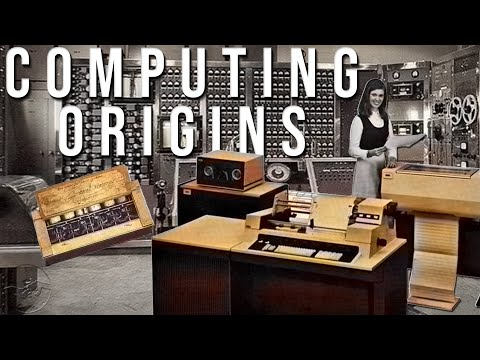
\includegraphics[keepaspectratio]{/Users/caballero/repos/teaching/modern-classical-mechanics/images/notes/week2/-M6lANfzFsM.jpg}}}

Source: \url{https://www.youtube.com/watch?v=-M6lANfzFsM}

    \subsection{A Critical Perspective on
Computing}\label{a-critical-perspective-on-computing}

While the history of computing is often celebrated as a story of
innovation, it is deeply entangled with systems of power, exploitation,
and violence. Computing technologies have not only been tools of
scientific progress but also instruments for surveillance, war, and
perpetuation of systemic biases.

```\{admonition\} Humans as Computers :class: note

Of course, the development of electronic computers was a huge
development for science. Prior to that, humans were employed to do the
calculations that we now do with computational algorithms. This work
occurred in a wide variety of labs where data were entered into tables,
calculations were done by hand, and the results were tabulated manually.

Frequently the work was done by those with less power in the laboratory
and broader society (e.g., women, immigrants, and folks of color). A
notable and well-known example is the work of the
\href{https://en.wikipedia.org/wiki/Harvard_Computers}{Harvard
Computers} in the late 19th and early 20th centuries where women were
employed to do the calculations that led to significant discoveries in
astronomy.

\begin{figure}
\centering
\pandocbounded{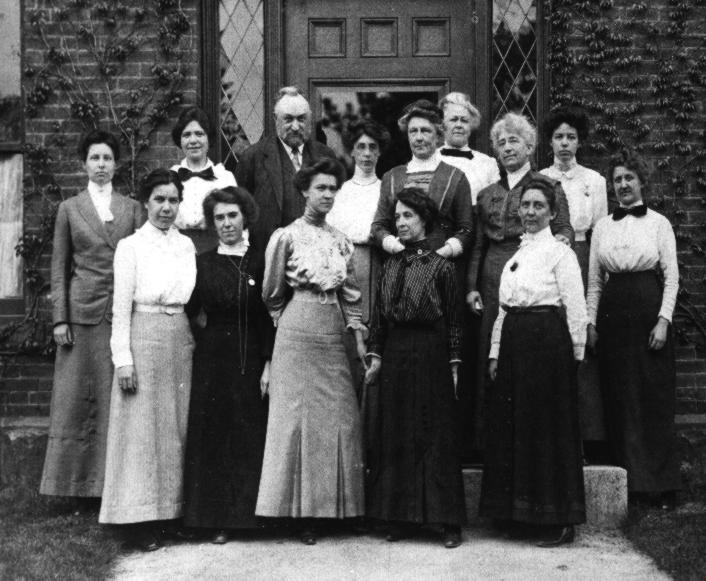
\includegraphics[keepaspectratio,alt={Harvard Computers}]{/Users/caballero/repos/teaching/modern-classical-mechanics/images/notes/week2/harvard-computers.png}}
\caption{Harvard Computers}
\end{figure}

One of the most important examples is the work done by African-American
women at NASA in the 1960s, as depicted in the book and movie
\href{https://en.wikipedia.org/wiki/Hidden_Figures}{Hidden Figures}.

\begin{figure}
\centering
\pandocbounded{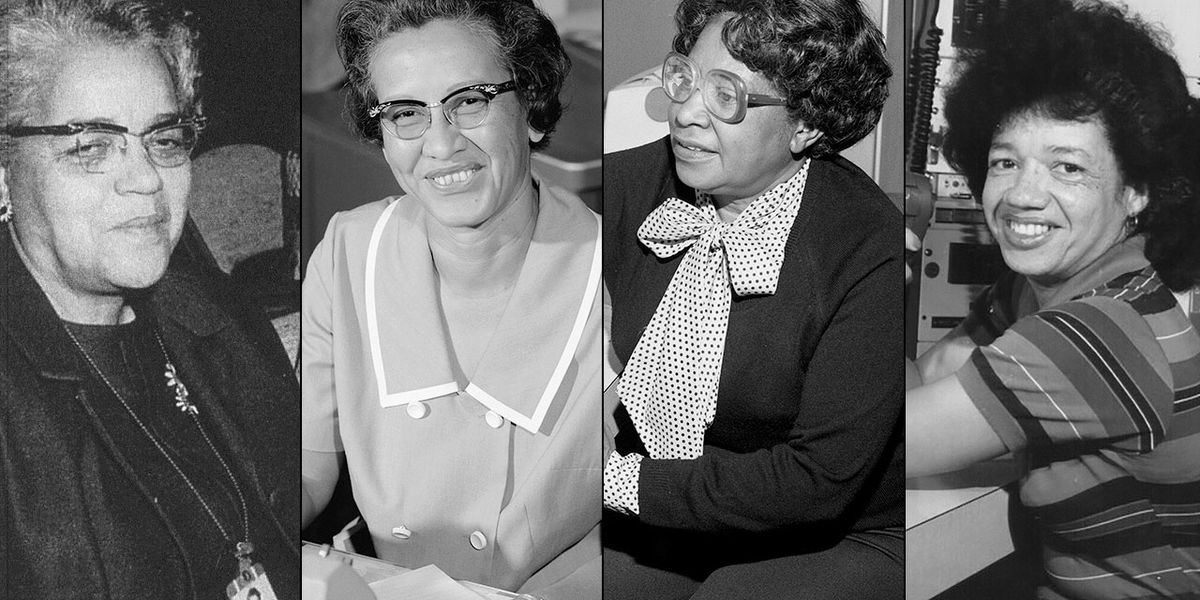
\includegraphics[keepaspectratio,alt={Hidden Figures}]{/Users/caballero/repos/teaching/modern-classical-mechanics/images/notes/week2/nasa-computers-hidden-figures.png}}
\caption{Hidden Figures}
\end{figure}

Women highlighted in this work include:
\href{https://en.wikipedia.org/wiki/Williamina_Fleming}{Williamina
Fleming}, \href{https://en.wikipedia.org/wiki/Florence_Cushman}{Florence
Cushman},
\href{https://en.wikipedia.org/wiki/Katherine_Johnson}{Katherine
Johnson}, \href{https://en.wikipedia.org/wiki/Dorothy_Vaughan}{Dorothy
Vaughan}, and \href{https://en.wikipedia.org/wiki/Mary_Jackson}{Mary
Jackson}. ```

The algorithms driving modern computing are not neutral---they reflect
the biases of the societies that create them. In
\href{https://www.penguinrandomhouse.com/books/241363/weapons-of-math-destruction-by-cathy-oneil/}{Cathy
O'Neil's \emph{Weapons of Math Destruction}}, the author explores how
algorithms used in areas like policing, hiring, and education often
reinforce systemic inequality, disproportionately harming marginalized
communities. Similarly,
\href{https://www.ruhabenjamin.com/race-after-technology}{Ruha
Benjamin's \emph{Race After Technology}} examines how race and
technology intersect, showing how seemingly ``objective'' systems encode
and perpetuate racial biases.

The use of AI in policing is another area of concern.
\href{https://www.dukeupress.edu/dark-matters}{Simone Browne's
\emph{Dark Matters}} highlights how surveillance technologies, from
facial recognition to predictive policing, are rooted in practices of
racialized social control, extending systems of oppression into the
digital realm.

The militarization of AI is one of the most alarming developments in
computing. AI-driven drones and autonomous weapons, often described as
the future of warfare, raise profound ethical and humanitarian concerns.
\href{https://shoshanazuboff.com/book/about/}{Shoshana Zuboff's
\emph{The Age of Surveillance Capitalism}} discusses how the same
technologies used for corporate profit are repurposed for state
surveillance and military applications, blurring the lines between
civilian and combatant spaces.

Additionally,
\href{https://peterasaro.org/writing/Asaro\%20Oxford\%20AI\%20Ethics\%20AWS.pdf}{Peter
Asaro's work on lethal autonomous weapons} questions the morality and
legality of machines making life-and-death decisions. Meanwhile,
\href{https://katecrawford.net/atlas}{Kate Crawford's \emph{Atlas of
AI}} explores how AI systems, from mining rare earth materials to
deployment in warfare, are deeply intertwined with colonial exploitation
and ecological destruction.

The tech industry's focus on profit has devastating environmental and
social impacts. Computing relies on the extraction of rare materials,
energy-intensive processes, and exploitative labor practices.
\href{https://thischangeseverything.org/}{Naomi Klein's \emph{This
Changes Everything}} examines how capitalism exacerbates climate change,
with insights into the environmental toll of computing technologies.
\href{https://cup.columbia.edu/book/artificial-whiteness/9780231194914}{Yarden
Katz's \emph{Artificial Whiteness}} connects the development of AI to
broader systems of capitalist and racial oppression.

    \subsection{Additional Resources for
Exploration}\label{additional-resources-for-exploration}

For deeper dives into these ideas, consider the following materials:

\begin{longtable}[]{@{}
  >{\raggedright\arraybackslash}p{(\linewidth - 2\tabcolsep) * \real{0.4348}}
  >{\raggedright\arraybackslash}p{(\linewidth - 2\tabcolsep) * \real{0.5652}}@{}}
\toprule\noalign{}
\begin{minipage}[b]{\linewidth}\raggedright
Resource
\end{minipage} & \begin{minipage}[b]{\linewidth}\raggedright
Description
\end{minipage} \\
\midrule\noalign{}
\endhead
\bottomrule\noalign{}
\endlastfoot
\href{https://www.penguinrandomhouse.com/books/44425/turings-cathedral-by-george-dyson/}{George
Dyson's \emph{Turing's Cathedral}}
\pandocbounded{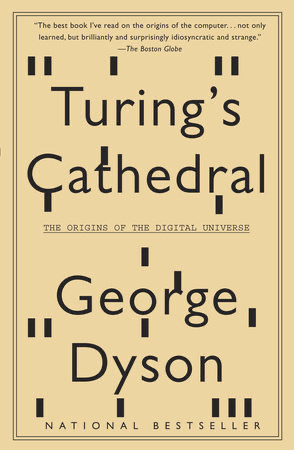
\includegraphics[keepaspectratio,alt={Turing's Cathedral}]{/Users/caballero/repos/teaching/modern-classical-mechanics/images/notes/week2/dyson.png}}
& Chronicles the origins of the modern computer, focusing on
\href{https://en.wikipedia.org/wiki/John_von_Neumann}{John von Neumann}
and his team at Princeton in the 1940s. This book delves into the
intersection of mathematics, physics, and computation, highlighting the
development of the first stored-program computers and their role in
shaping the digital age. \\
\href{https://www.penguinrandomhouse.com/books/60765/the-information-by-james-gleick/}{James
Gleick's \emph{The Information}}
\pandocbounded{
\includegraphics[keepaspectratio,alt={The Information}]{/Users/caballero/repos/teaching/modern-classical-mechanics/images/notes/week2/gleick.png}}
& Explores the transformative impact of information theory on science,
technology, and culture. From the invention of writing to the digital
age, Gleick highlights key figures like Michigander
\href{https://en.wikipedia.org/wiki/Claude_Shannon}{Claude Shannon}, who
revolutionized communication with his groundbreaking mathematical theory
of information. \\
\href{https://www.stevenlevy.com/hackers-heroes-of-the-computer-revolution}{Steven
Levy's \emph{Hackers}}
\pandocbounded{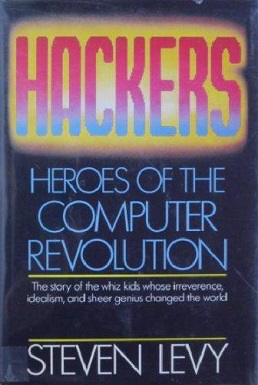
\includegraphics[keepaspectratio,alt={Hackers}]{/Users/caballero/repos/teaching/modern-classical-mechanics/images/notes/week2/levy.png}}
& Chronicles the rise of hacker culture, from early computer pioneers to
the creators of the personal computer revolution. Levy examines the
``hacker ethic,'' emphasizing creativity, open access, and the joy of
problem-solving, which shaped the tools and technologies we use
today. \\
\href{https://www.penguinrandomhouse.com/books/241363/weapons-of-math-destruction-by-cathy-oneil/}{Cathy
O'Neil's \emph{Weapons of Math Destruction}}
\pandocbounded{
\includegraphics[keepaspectratio,alt={Weapons of Math Destruction}]{/Users/caballero/repos/teaching/modern-classical-mechanics/images/notes/week2/oneill.png}}
& Explores how algorithms, often marketed as objective, exacerbate
inequality in policing, hiring, and credit scoring. O'Neil critically
examines the dangers of data-driven systems that disproportionately harm
marginalized communities while remaining opaque and unregulated. \\
\href{https://www.ruhabenjamin.com/race-after-technology}{Ruha
Benjamin's \emph{Race After Technology}}
\pandocbounded{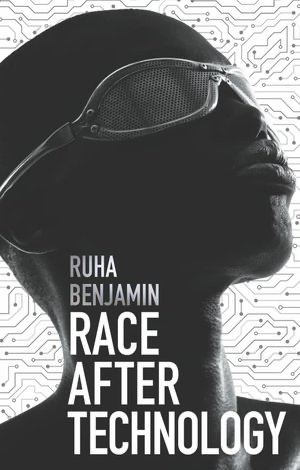
\includegraphics[keepaspectratio,alt={Race After Technology}]{/Users/caballero/repos/teaching/modern-classical-mechanics/images/notes/week2/benjamin.png}}
& Analyzes how algorithms and technologies reinforce systemic racism
under the guise of neutrality. Benjamin introduces the concept of the
``New Jim Code,'' highlighting the ways in which technological tools
amplify inequities while appearing fair and impartial. \\
\href{https://www.dukeupress.edu/dark-matters}{Simone Browne's
\emph{Dark Matters}}
\pandocbounded{
\includegraphics[keepaspectratio,alt={Dark Matters}]{/Users/caballero/repos/teaching/modern-classical-mechanics/images/notes/week2/browne.png}}
& Examines how surveillance technologies are deeply rooted in practices
of racialized social control. Browne connects historical practices like
slave surveillance to modern tools like facial recognition and
predictive policing, revealing the persistence of systemic inequities in
new forms. \\
\href{https://katecrawford.net/atlas}{Kate Crawford's \emph{Atlas of
AI}}
\pandocbounded{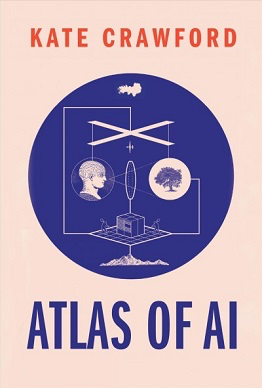
\includegraphics[keepaspectratio,alt={Atlas of AI}]{/Users/caballero/repos/teaching/modern-classical-mechanics/images/notes/week2/crawford.png}}
& Explores the hidden costs of artificial intelligence, from resource
extraction to labor exploitation and military applications. Crawford
critiques AI as an extractive industry that reshapes power dynamics and
perpetuates global inequalities while causing significant environmental
damage. \\
\href{https://shoshanazuboff.com/book/about/}{Shoshana Zuboff's
\emph{The Age of Surveillance Capitalism}}
\pandocbounded{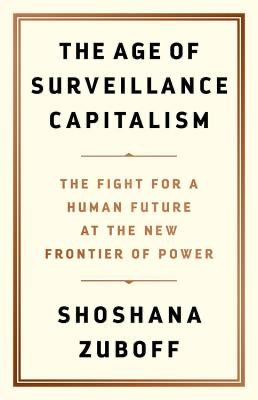
\includegraphics[keepaspectratio,alt={Age of Surveillance Capitalism}]{/Users/caballero/repos/teaching/modern-classical-mechanics/images/notes/week2/zuboff.png}}
& Investigates how corporations and governments exploit personal data
for profit and control. Zuboff coins the term ``surveillance
capitalism'' to describe how the tech industry commodifies human
behavior, eroding privacy and autonomy while reshaping society's power
structures. \\
\end{longtable}

    

    

    

    


    % Add a bibliography block to the postdoc
    
    
    
\end{document}
